% Options for packages loaded elsewhere
\PassOptionsToPackage{unicode}{hyperref}
\PassOptionsToPackage{hyphens}{url}
%
\documentclass[
]{article}
\usepackage{lmodern}
\usepackage{amssymb,amsmath}
\usepackage{ifxetex,ifluatex}
\ifnum 0\ifxetex 1\fi\ifluatex 1\fi=0 % if pdftex
  \usepackage[T1]{fontenc}
  \usepackage[utf8]{inputenc}
  \usepackage{textcomp} % provide euro and other symbols
\else % if luatex or xetex
  \usepackage{unicode-math}
  \defaultfontfeatures{Scale=MatchLowercase}
  \defaultfontfeatures[\rmfamily]{Ligatures=TeX,Scale=1}
\fi
% Use upquote if available, for straight quotes in verbatim environments
\IfFileExists{upquote.sty}{\usepackage{upquote}}{}
\IfFileExists{microtype.sty}{% use microtype if available
  \usepackage[]{microtype}
  \UseMicrotypeSet[protrusion]{basicmath} % disable protrusion for tt fonts
}{}
\makeatletter
\@ifundefined{KOMAClassName}{% if non-KOMA class
  \IfFileExists{parskip.sty}{%
    \usepackage{parskip}
  }{% else
    \setlength{\parindent}{0pt}
    \setlength{\parskip}{6pt plus 2pt minus 1pt}}
}{% if KOMA class
  \KOMAoptions{parskip=half}}
\makeatother
\usepackage{xcolor}
\IfFileExists{xurl.sty}{\usepackage{xurl}}{} % add URL line breaks if available
\IfFileExists{bookmark.sty}{\usepackage{bookmark}}{\usepackage{hyperref}}
\hypersetup{
  pdftitle={Final\_Project},
  hidelinks,
  pdfcreator={LaTeX via pandoc}}
\urlstyle{same} % disable monospaced font for URLs
\usepackage[margin=1in]{geometry}
\usepackage{color}
\usepackage{fancyvrb}
\newcommand{\VerbBar}{|}
\newcommand{\VERB}{\Verb[commandchars=\\\{\}]}
\DefineVerbatimEnvironment{Highlighting}{Verbatim}{commandchars=\\\{\}}
% Add ',fontsize=\small' for more characters per line
\usepackage{framed}
\definecolor{shadecolor}{RGB}{248,248,248}
\newenvironment{Shaded}{\begin{snugshade}}{\end{snugshade}}
\newcommand{\AlertTok}[1]{\textcolor[rgb]{0.94,0.16,0.16}{#1}}
\newcommand{\AnnotationTok}[1]{\textcolor[rgb]{0.56,0.35,0.01}{\textbf{\textit{#1}}}}
\newcommand{\AttributeTok}[1]{\textcolor[rgb]{0.77,0.63,0.00}{#1}}
\newcommand{\BaseNTok}[1]{\textcolor[rgb]{0.00,0.00,0.81}{#1}}
\newcommand{\BuiltInTok}[1]{#1}
\newcommand{\CharTok}[1]{\textcolor[rgb]{0.31,0.60,0.02}{#1}}
\newcommand{\CommentTok}[1]{\textcolor[rgb]{0.56,0.35,0.01}{\textit{#1}}}
\newcommand{\CommentVarTok}[1]{\textcolor[rgb]{0.56,0.35,0.01}{\textbf{\textit{#1}}}}
\newcommand{\ConstantTok}[1]{\textcolor[rgb]{0.00,0.00,0.00}{#1}}
\newcommand{\ControlFlowTok}[1]{\textcolor[rgb]{0.13,0.29,0.53}{\textbf{#1}}}
\newcommand{\DataTypeTok}[1]{\textcolor[rgb]{0.13,0.29,0.53}{#1}}
\newcommand{\DecValTok}[1]{\textcolor[rgb]{0.00,0.00,0.81}{#1}}
\newcommand{\DocumentationTok}[1]{\textcolor[rgb]{0.56,0.35,0.01}{\textbf{\textit{#1}}}}
\newcommand{\ErrorTok}[1]{\textcolor[rgb]{0.64,0.00,0.00}{\textbf{#1}}}
\newcommand{\ExtensionTok}[1]{#1}
\newcommand{\FloatTok}[1]{\textcolor[rgb]{0.00,0.00,0.81}{#1}}
\newcommand{\FunctionTok}[1]{\textcolor[rgb]{0.00,0.00,0.00}{#1}}
\newcommand{\ImportTok}[1]{#1}
\newcommand{\InformationTok}[1]{\textcolor[rgb]{0.56,0.35,0.01}{\textbf{\textit{#1}}}}
\newcommand{\KeywordTok}[1]{\textcolor[rgb]{0.13,0.29,0.53}{\textbf{#1}}}
\newcommand{\NormalTok}[1]{#1}
\newcommand{\OperatorTok}[1]{\textcolor[rgb]{0.81,0.36,0.00}{\textbf{#1}}}
\newcommand{\OtherTok}[1]{\textcolor[rgb]{0.56,0.35,0.01}{#1}}
\newcommand{\PreprocessorTok}[1]{\textcolor[rgb]{0.56,0.35,0.01}{\textit{#1}}}
\newcommand{\RegionMarkerTok}[1]{#1}
\newcommand{\SpecialCharTok}[1]{\textcolor[rgb]{0.00,0.00,0.00}{#1}}
\newcommand{\SpecialStringTok}[1]{\textcolor[rgb]{0.31,0.60,0.02}{#1}}
\newcommand{\StringTok}[1]{\textcolor[rgb]{0.31,0.60,0.02}{#1}}
\newcommand{\VariableTok}[1]{\textcolor[rgb]{0.00,0.00,0.00}{#1}}
\newcommand{\VerbatimStringTok}[1]{\textcolor[rgb]{0.31,0.60,0.02}{#1}}
\newcommand{\WarningTok}[1]{\textcolor[rgb]{0.56,0.35,0.01}{\textbf{\textit{#1}}}}
\usepackage{graphicx,grffile}
\makeatletter
\def\maxwidth{\ifdim\Gin@nat@width>\linewidth\linewidth\else\Gin@nat@width\fi}
\def\maxheight{\ifdim\Gin@nat@height>\textheight\textheight\else\Gin@nat@height\fi}
\makeatother
% Scale images if necessary, so that they will not overflow the page
% margins by default, and it is still possible to overwrite the defaults
% using explicit options in \includegraphics[width, height, ...]{}
\setkeys{Gin}{width=\maxwidth,height=\maxheight,keepaspectratio}
% Set default figure placement to htbp
\makeatletter
\def\fps@figure{htbp}
\makeatother
\setlength{\emergencystretch}{3em} % prevent overfull lines
\providecommand{\tightlist}{%
  \setlength{\itemsep}{0pt}\setlength{\parskip}{0pt}}
\setcounter{secnumdepth}{-\maxdimen} % remove section numbering

\title{Final\_Project}
\author{}
\date{\vspace{-2.5em}}

\begin{document}
\maketitle

\hypertarget{home-about-me-cv-programming-research-exam-3}{%
\subsection{\texorpdfstring{\href{http://MurderousPolyhedron.github.io/}{HOME}
\textbar{} \href{http://MurderousPolyhedron.github.io/About_Me/}{ABOUT
ME} \textbar{} \href{http://MurderousPolyhedron.github.io/CV/}{CV}
\textbar{}
\href{http://MurderousPolyhedron.github.io/Programming/}{PROGRAMMING}
\textbar{}
\href{http://MurderousPolyhedron.github.io/Research/}{RESEARCH}
\textbar{} \href{http://MurderousPolyhedron.github.io/Exam_3/}{Exam
3}}{HOME \textbar{} ABOUT ME \textbar{} CV \textbar{} PROGRAMMING \textbar{} RESEARCH \textbar{} Exam 3}}\label{home-about-me-cv-programming-research-exam-3}}

\hypertarget{before-we-start-off-on-this-here-is-the-initial-code-of-tidying-some-of-the-data.-now-you-may-be-asking-why-isnt-this-just-in-the-code-well-the-initial-data-was-286.07mb-big-even-when-compressing-it-into-a-zip-file-it-was-still-199mb-large.-so-obviously-these-files-are-much-to-large-to-put-on-github-without-paying-their-premium-service.-as-a-college-student-i-cant-justify-that-cost.-so-i-will-be-providing-the-initial-code-to-demonstrate-what-i-did-to-tidy-the-data-into-a-much-more-manageable-size-along-with-a-link-to-download-the-original-dataset.-the-raw-data-can-be-found-here-httpsdrive.google.comopenid1mbg2a-vqttclhgn8-pcwirx3cb7xzb0_-and-here-is-the-code.}{%
\subsubsection{\texorpdfstring{Before we start off on this here is the
initial code of tidying some of the data. Now you may be asking why
isn't this just in the code? Well the initial data was 286.07mb big,
even when compressing it into a zip file it was still 199mb large. So
obviously these files are much to large to put on github without paying
their premium service. As a college student I can't justify that cost.
So I will be providing the initial code to demonstrate what I did to
tidy the data into a much more manageable size along with a link to
download the original dataset. The raw data can be found here
\url{https://drive.google.com/open?id=1MbG2a-vQtTclHgn8-PCwIrx3CB7xzb0_}
, and here is the
code.}{Before we start off on this here is the initial code of tidying some of the data. Now you may be asking why isn't this just in the code? Well the initial data was 286.07mb big, even when compressing it into a zip file it was still 199mb large. So obviously these files are much to large to put on github without paying their premium service. As a college student I can't justify that cost. So I will be providing the initial code to demonstrate what I did to tidy the data into a much more manageable size along with a link to download the original dataset. The raw data can be found here https://drive.google.com/open?id=1MbG2a-vQtTclHgn8-PCwIrx3CB7xzb0\_ , and here is the code.}}\label{before-we-start-off-on-this-here-is-the-initial-code-of-tidying-some-of-the-data.-now-you-may-be-asking-why-isnt-this-just-in-the-code-well-the-initial-data-was-286.07mb-big-even-when-compressing-it-into-a-zip-file-it-was-still-199mb-large.-so-obviously-these-files-are-much-to-large-to-put-on-github-without-paying-their-premium-service.-as-a-college-student-i-cant-justify-that-cost.-so-i-will-be-providing-the-initial-code-to-demonstrate-what-i-did-to-tidy-the-data-into-a-much-more-manageable-size-along-with-a-link-to-download-the-original-dataset.-the-raw-data-can-be-found-here-httpsdrive.google.comopenid1mbg2a-vqttclhgn8-pcwirx3cb7xzb0_-and-here-is-the-code.}}

\begin{verbatim}
library(lubridate)
library(tidyverse)
df <- read.csv("../UL_BiologicalData_1.csv")
class(df$ActivityStartDate)
df$ActivityStartDate <- as.Date(df$ActivityStartDate, format = "%m/%d/%Y")
df2 <- subset(df, ActivityStartDate > "2016-05-24" & ActivityStartDate < "2017-08-26")
df3 <- subset(df2,
              select = c("ActivityStartDate","ActivityStartTime.Time",
                         "ActivityEndDate","ActivityEndTime.Time",
                         "ActivityDepthHeightMeasure.MeasureValue",
                         "MonitoringLocationIdentifier",
                         "ActivityLocation.LatitudeMeasure",
                         "ActivityLocation.LongitudeMeasure"))
write.csv(df3,file = "../UL_BiologicalData_cleaned_2.csv")
\end{verbatim}

\begin{verbatim}
##  [1] "10147100"        "4996780"         "4996810"         "4996830"        
##  [5] "4996850"         "10166430"        "09312600"        "10163000"       
##  [9] "10149400"        "10150500"        "10153100"        "10149000"       
## [13] "10164500"        "401600112023401" "401702111594001" "4995640"        
## [17] "4995670"         "4995690"         "4995700"         "4995720"        
## [21] "4995780"         "395340111590001" "395956111572101" "400325111552501"
## [25] "401541111425001" "400423111454001" "401325111410901" "402133111484601"
## [29] "395717111512301" "401043111361801" "401539112045501" "401656112020301"
## [33] "402105111472601" "11"              "4994970"         "4995775"        
## [37] "4932830"         "4995710"         "4995760"         "401327111462601"
## [41] "401432111454301" "401613111463301" "401658111491601" "4996135"        
## [45] "401607112023401" "401730111594501" "4995680"         "4995925"        
## [49] "4995530"         "395942111470801" "4917310"         "4917320"        
## [53] "4917370"         "4917390"         "4917500"         "4917520"        
## [57] "4917770"         "400422111454201" "400407111375101" "402159111520101"
## [61] "402420111505701" "4995845"         "4995870"         "4995945"
\end{verbatim}

\begin{verbatim}
## Warning: NAs introduced by coercion
\end{verbatim}

\begin{verbatim}
##    Min. 1st Qu.  Median    Mean 3rd Qu.    Max.    NA's 
##    0.99    1.00    3.06  218.24  179.91 2419.57    5339
\end{verbatim}

\includegraphics{Final_Project_files/figure-latex/unnamed-chunk-6-1.pdf}

\begin{Shaded}
\begin{Highlighting}[]
\KeywordTok{ggplot}\NormalTok{(df3,}\KeywordTok{aes}\NormalTok{(}\DataTypeTok{x=}\NormalTok{Rain.Depth.Feet, }\DataTypeTok{y=}\StringTok{`}\DataTypeTok{E. coli MPN/100ml}\StringTok{`}\NormalTok{)) }\OperatorTok{+}
\StringTok{  }\KeywordTok{geom_point}\NormalTok{() }\OperatorTok{+}\StringTok{ }\KeywordTok{coord_cartesian}\NormalTok{(}\DataTypeTok{xlim =} \KeywordTok{c}\NormalTok{(}\DecValTok{0}\NormalTok{, }\DecValTok{4}\NormalTok{), }\DataTypeTok{ylim =} \KeywordTok{c}\NormalTok{(}\DecValTok{0}\NormalTok{, }\DecValTok{5}\NormalTok{))}
\end{Highlighting}
\end{Shaded}

\begin{verbatim}
## Warning: Removed 5867 rows containing missing values (geom_point).
\end{verbatim}

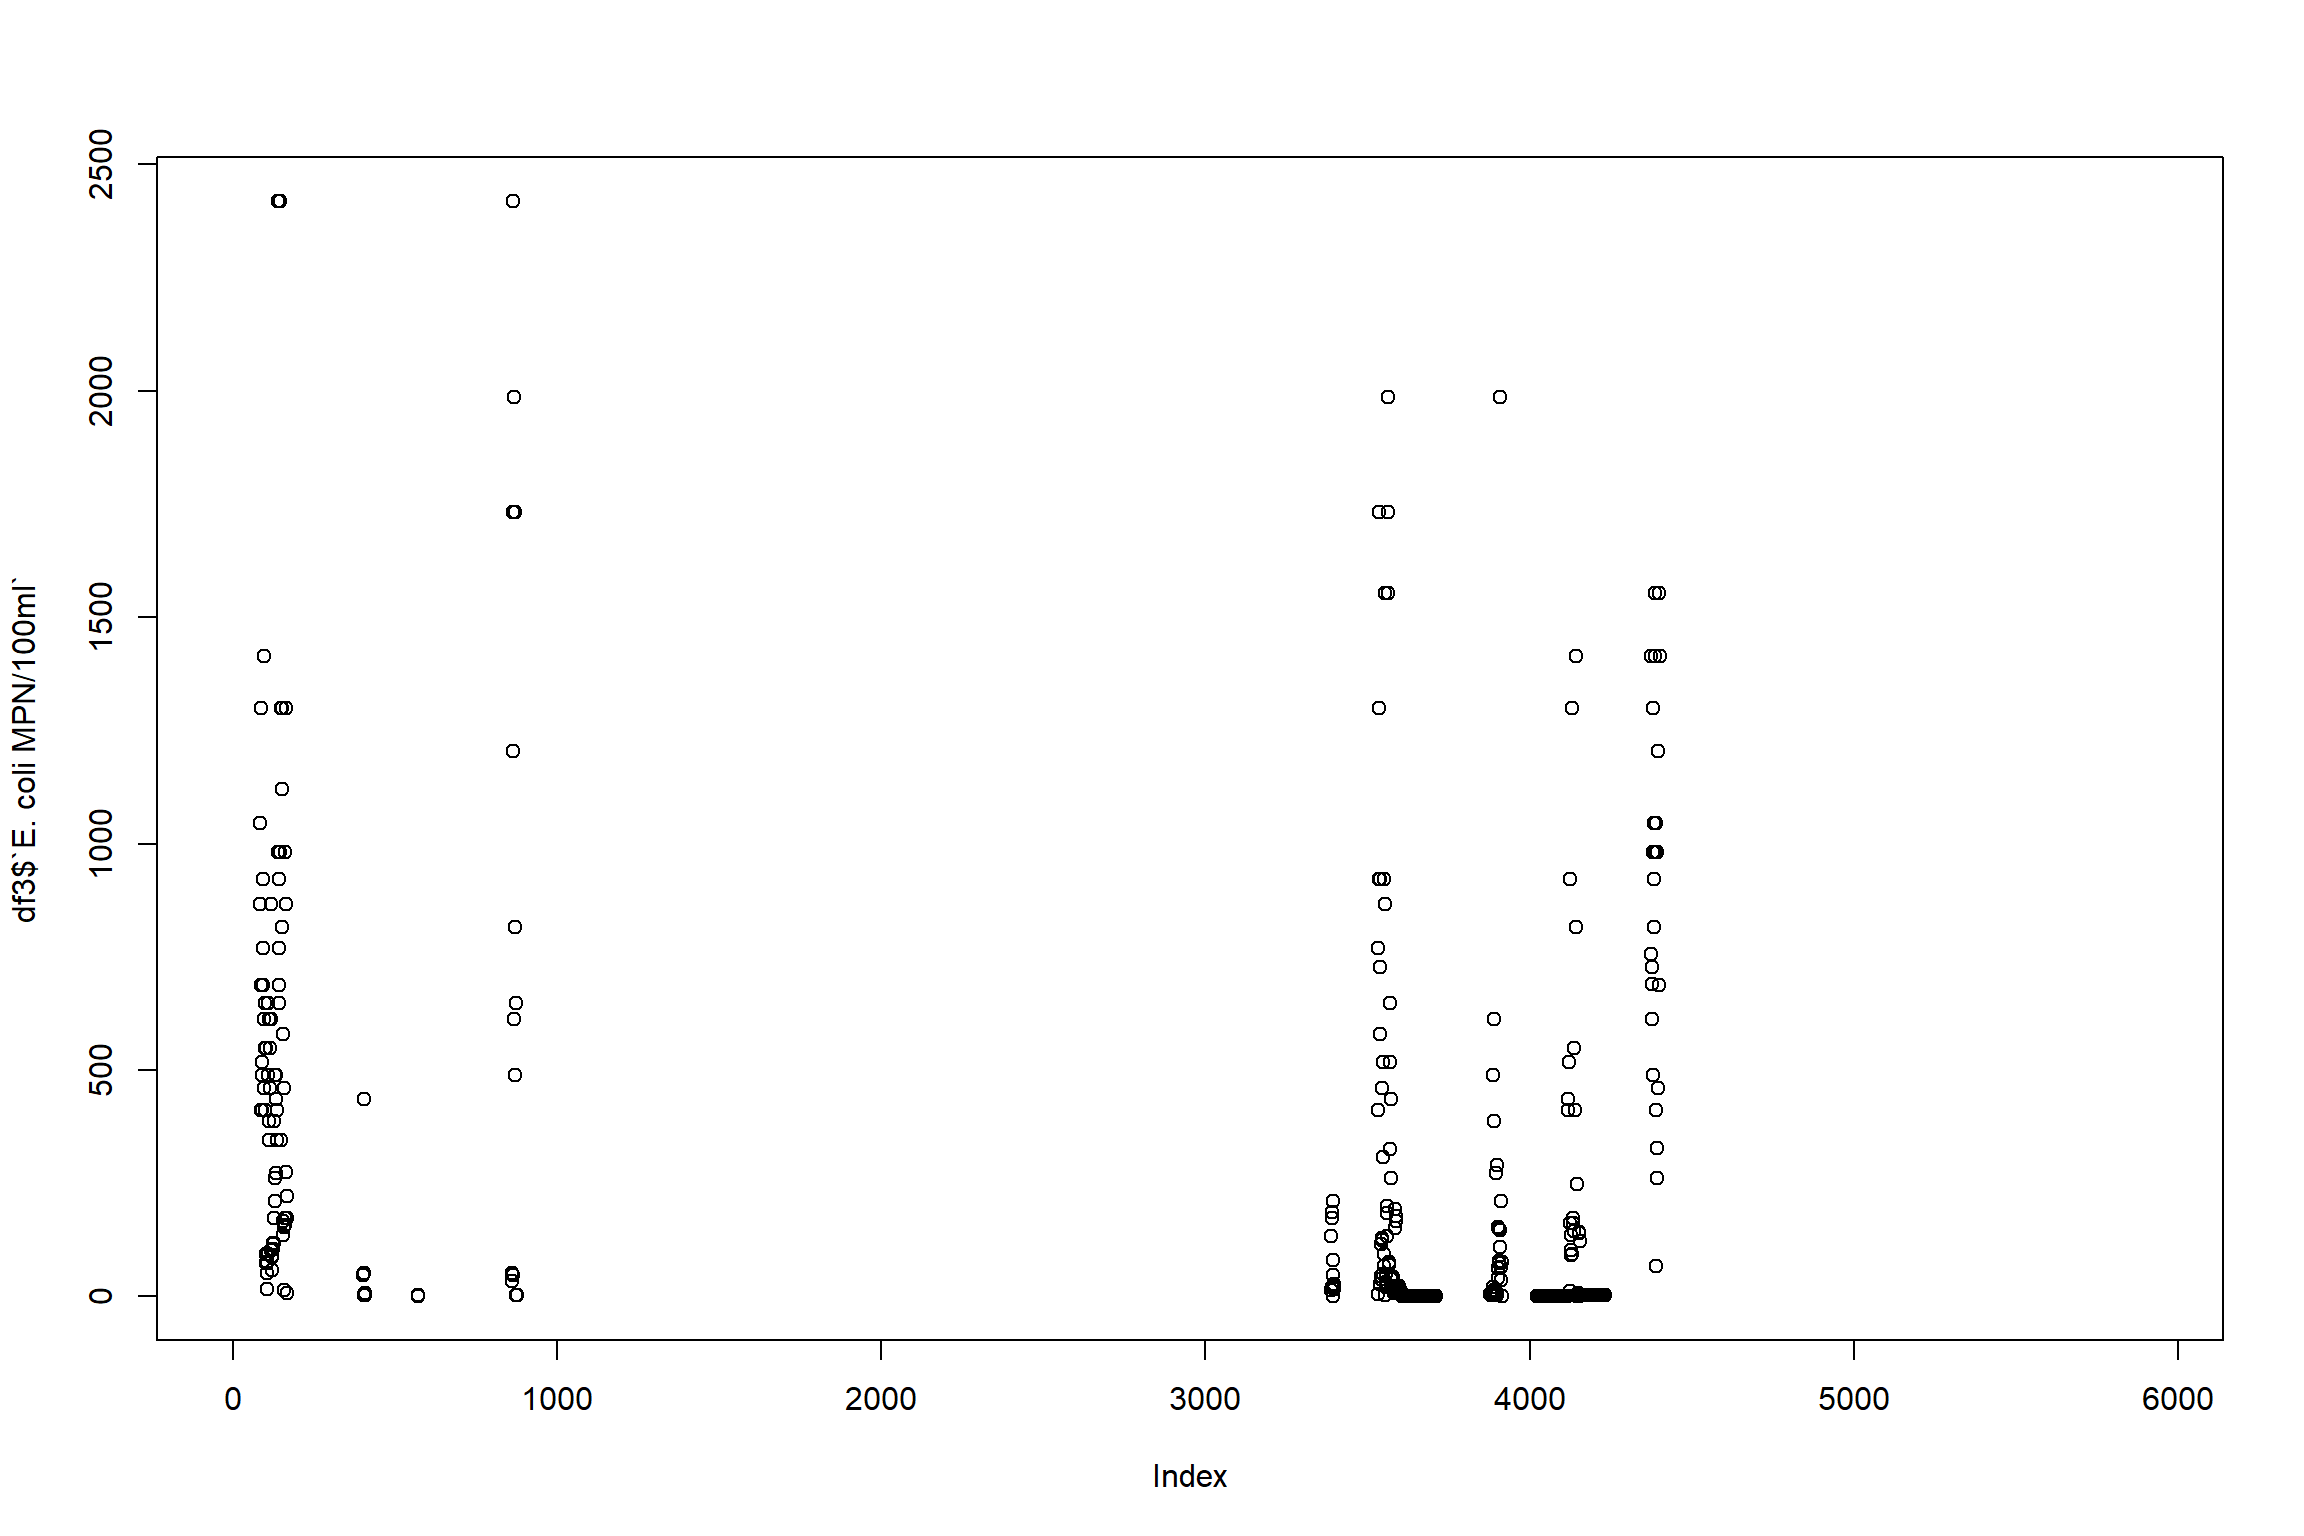
\includegraphics{Final_Project_files/figure-latex/unnamed-chunk-7-1.pdf}

\begin{Shaded}
\begin{Highlighting}[]
\KeywordTok{ggplot}\NormalTok{(df3,}\KeywordTok{aes}\NormalTok{(}\DataTypeTok{x=}\NormalTok{Rain.Depth.Feet, }\DataTypeTok{y=}\StringTok{`}\DataTypeTok{E. coli MPN/100ml}\StringTok{`}\NormalTok{)) }\OperatorTok{+}
\StringTok{  }\KeywordTok{geom_count}\NormalTok{() }\OperatorTok{+}\StringTok{ }\KeywordTok{coord_cartesian}\NormalTok{(}\DataTypeTok{xlim =} \KeywordTok{c}\NormalTok{(}\DecValTok{0}\NormalTok{, }\DecValTok{4}\NormalTok{), }\DataTypeTok{ylim =} \KeywordTok{c}\NormalTok{(}\DecValTok{0}\NormalTok{, }\DecValTok{5}\NormalTok{))}
\end{Highlighting}
\end{Shaded}

\begin{verbatim}
## Warning: Removed 5867 rows containing non-finite values (stat_sum).
\end{verbatim}

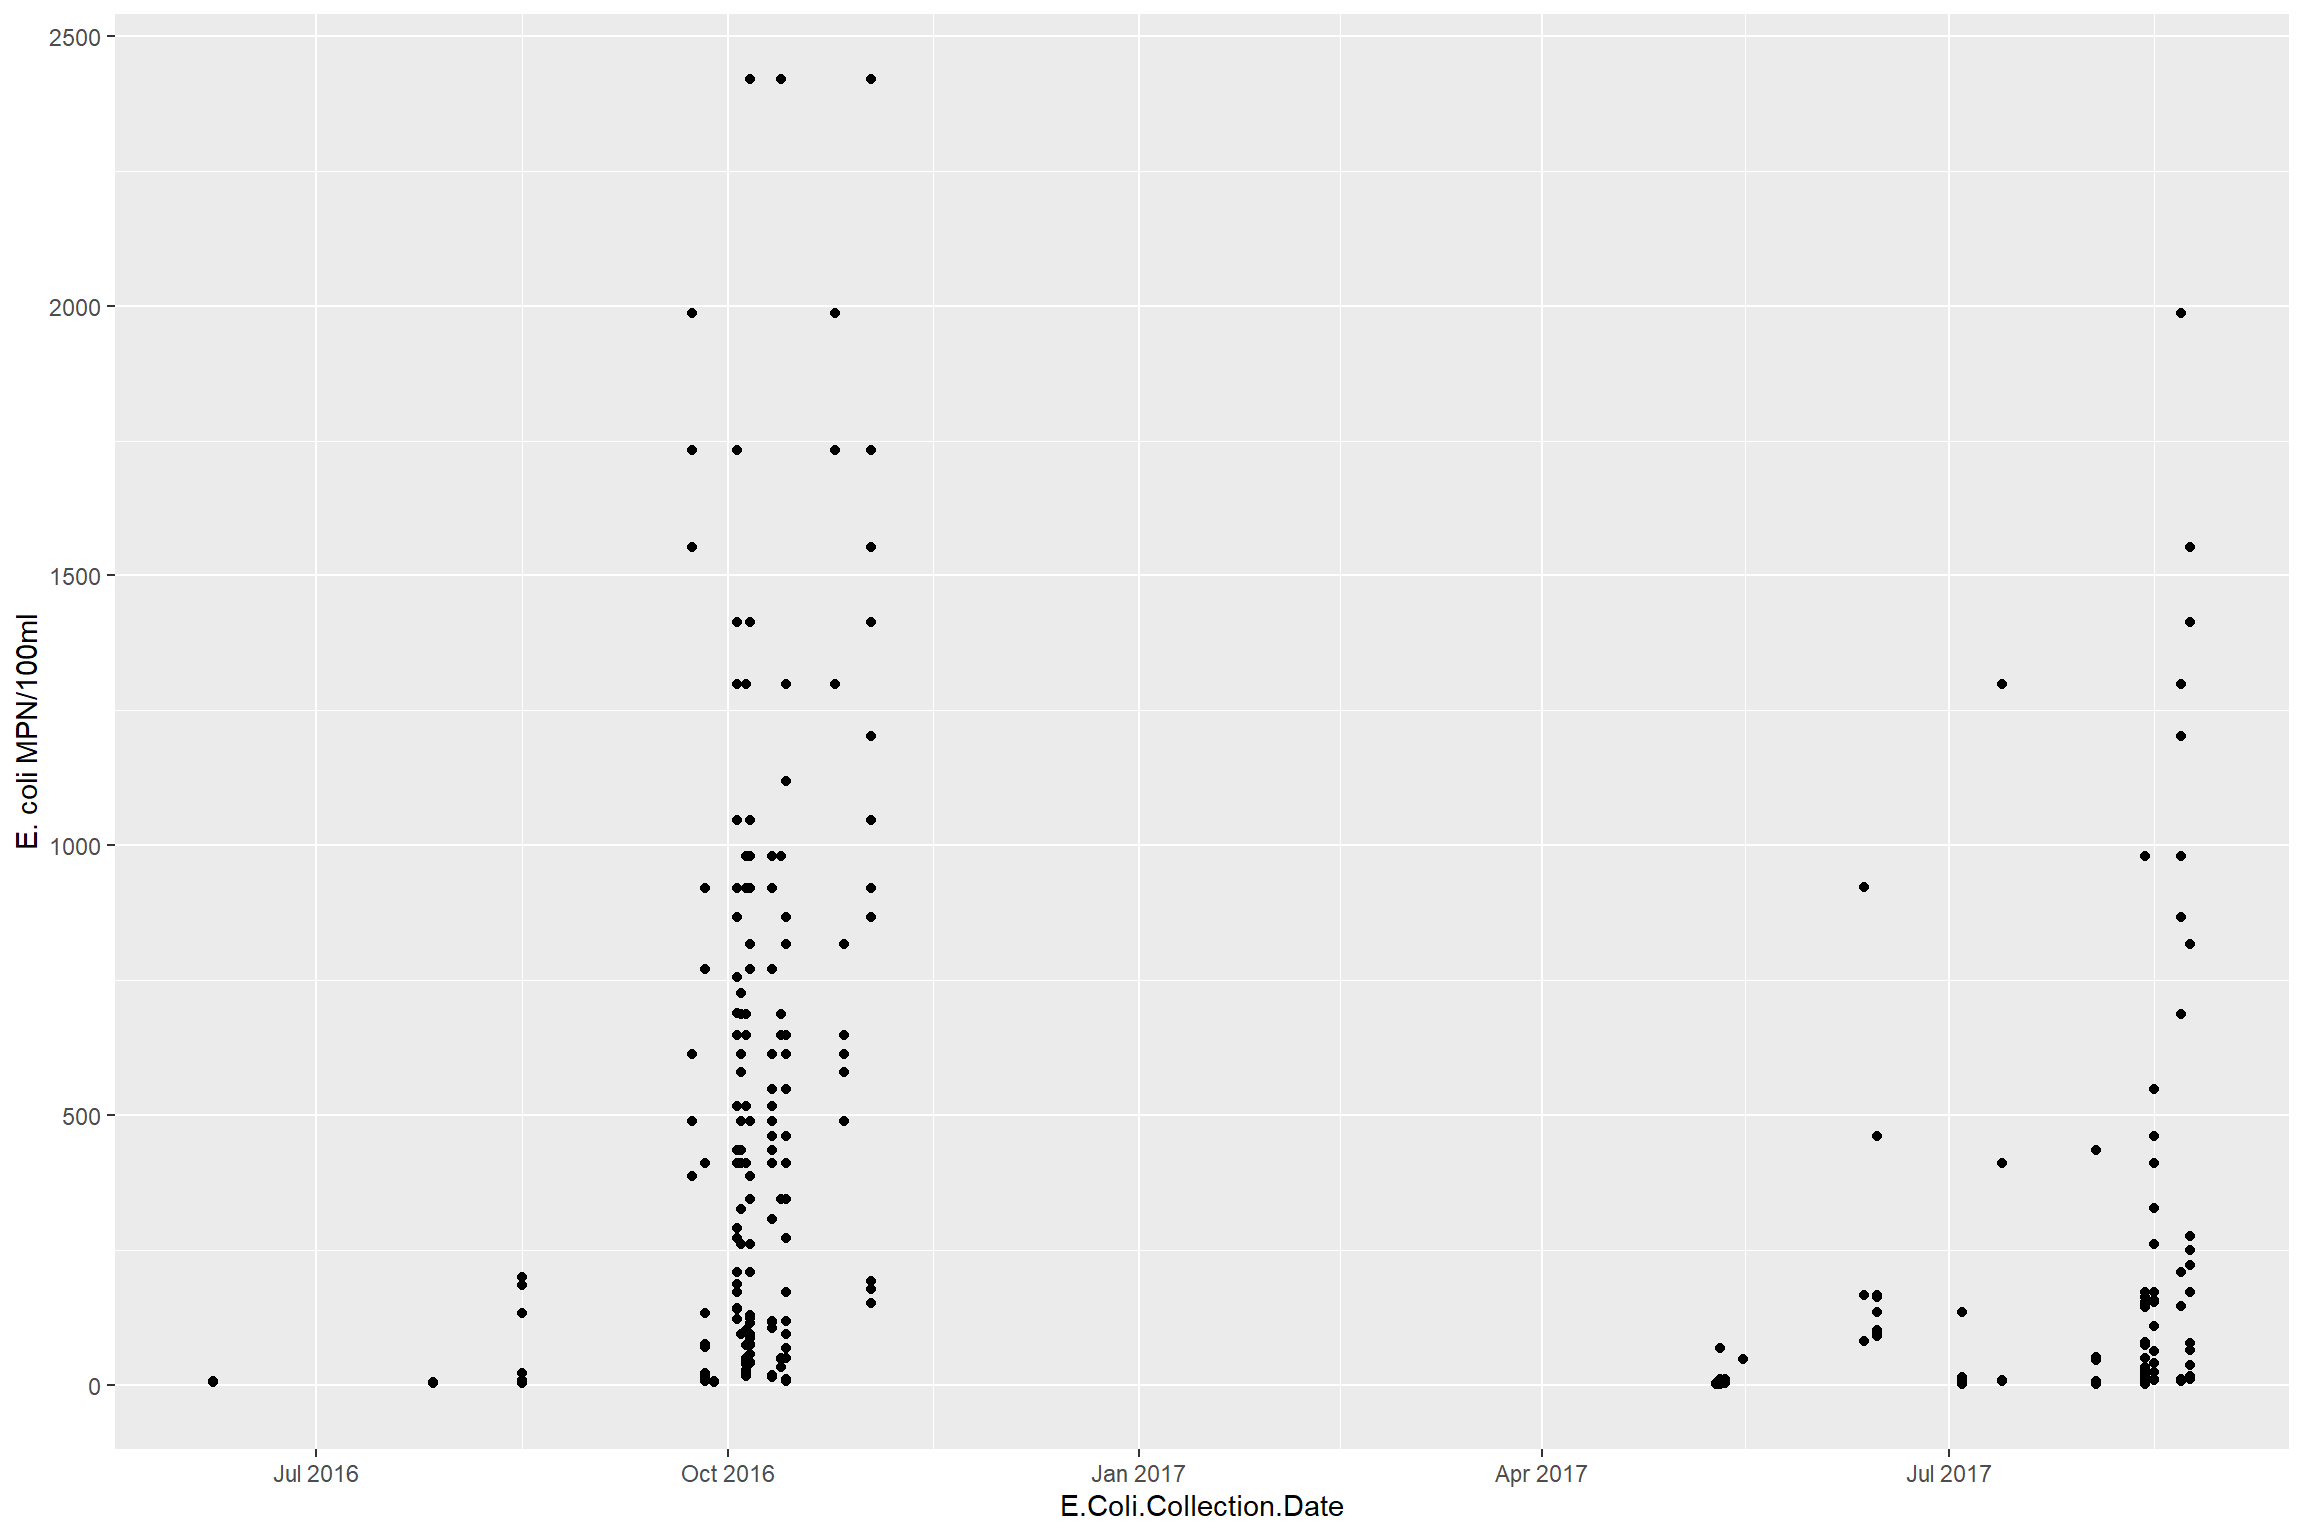
\includegraphics{Final_Project_files/figure-latex/unnamed-chunk-7-2.pdf}

\begin{Shaded}
\begin{Highlighting}[]
\KeywordTok{ggplot}\NormalTok{(df3,}\KeywordTok{aes}\NormalTok{(}\DataTypeTok{y=}\StringTok{`}\DataTypeTok{E. coli MPN/100ml}\StringTok{`}\NormalTok{, }\DataTypeTok{x=}\NormalTok{Rain.Start.Date)) }\OperatorTok{+}\StringTok{ }\KeywordTok{geom_point}\NormalTok{()}
\end{Highlighting}
\end{Shaded}

\begin{verbatim}
## Warning: Removed 5339 rows containing missing values (geom_point).
\end{verbatim}

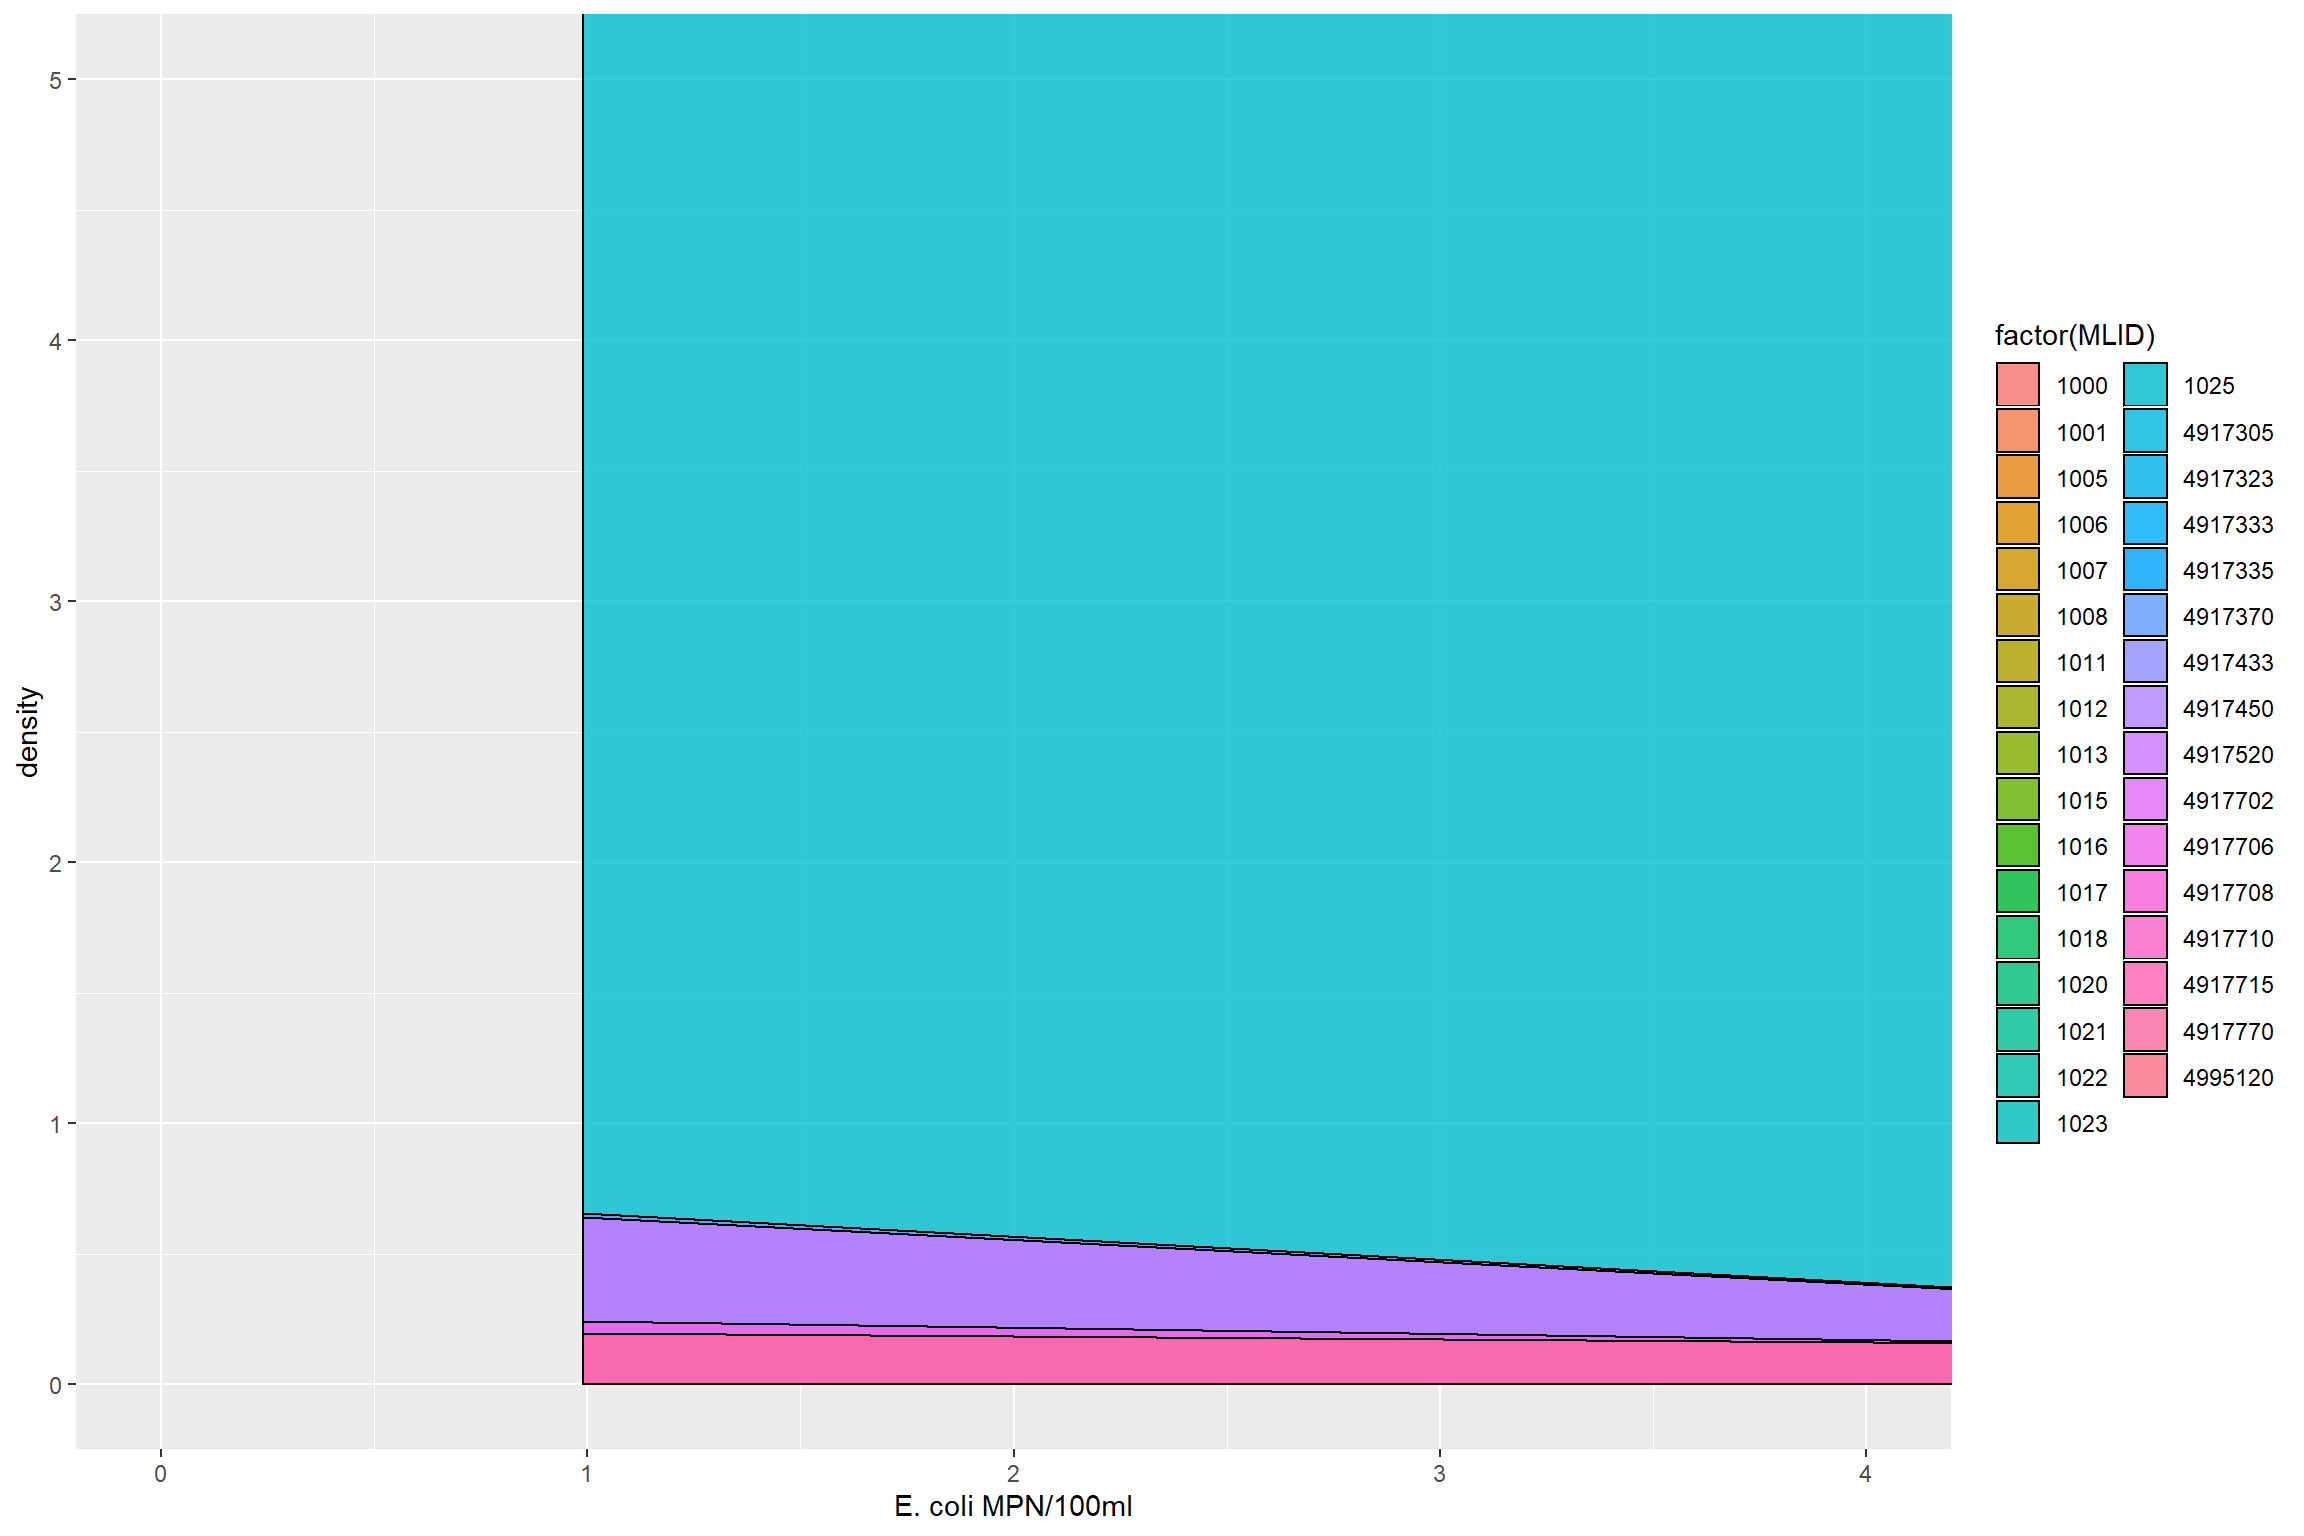
\includegraphics{Final_Project_files/figure-latex/unnamed-chunk-7-3.pdf}

\begin{Shaded}
\begin{Highlighting}[]
\KeywordTok{ggplot}\NormalTok{(df3,}\KeywordTok{aes}\NormalTok{(}\DataTypeTok{y=}\StringTok{`}\DataTypeTok{E. coli MPN/100ml}\StringTok{`}\NormalTok{, }\DataTypeTok{x=}\NormalTok{E.Coli.Collection.Date)) }\OperatorTok{+}\StringTok{ }\KeywordTok{geom_point}\NormalTok{()}
\end{Highlighting}
\end{Shaded}

\begin{verbatim}
## Warning: Removed 5339 rows containing missing values (geom_point).
\end{verbatim}

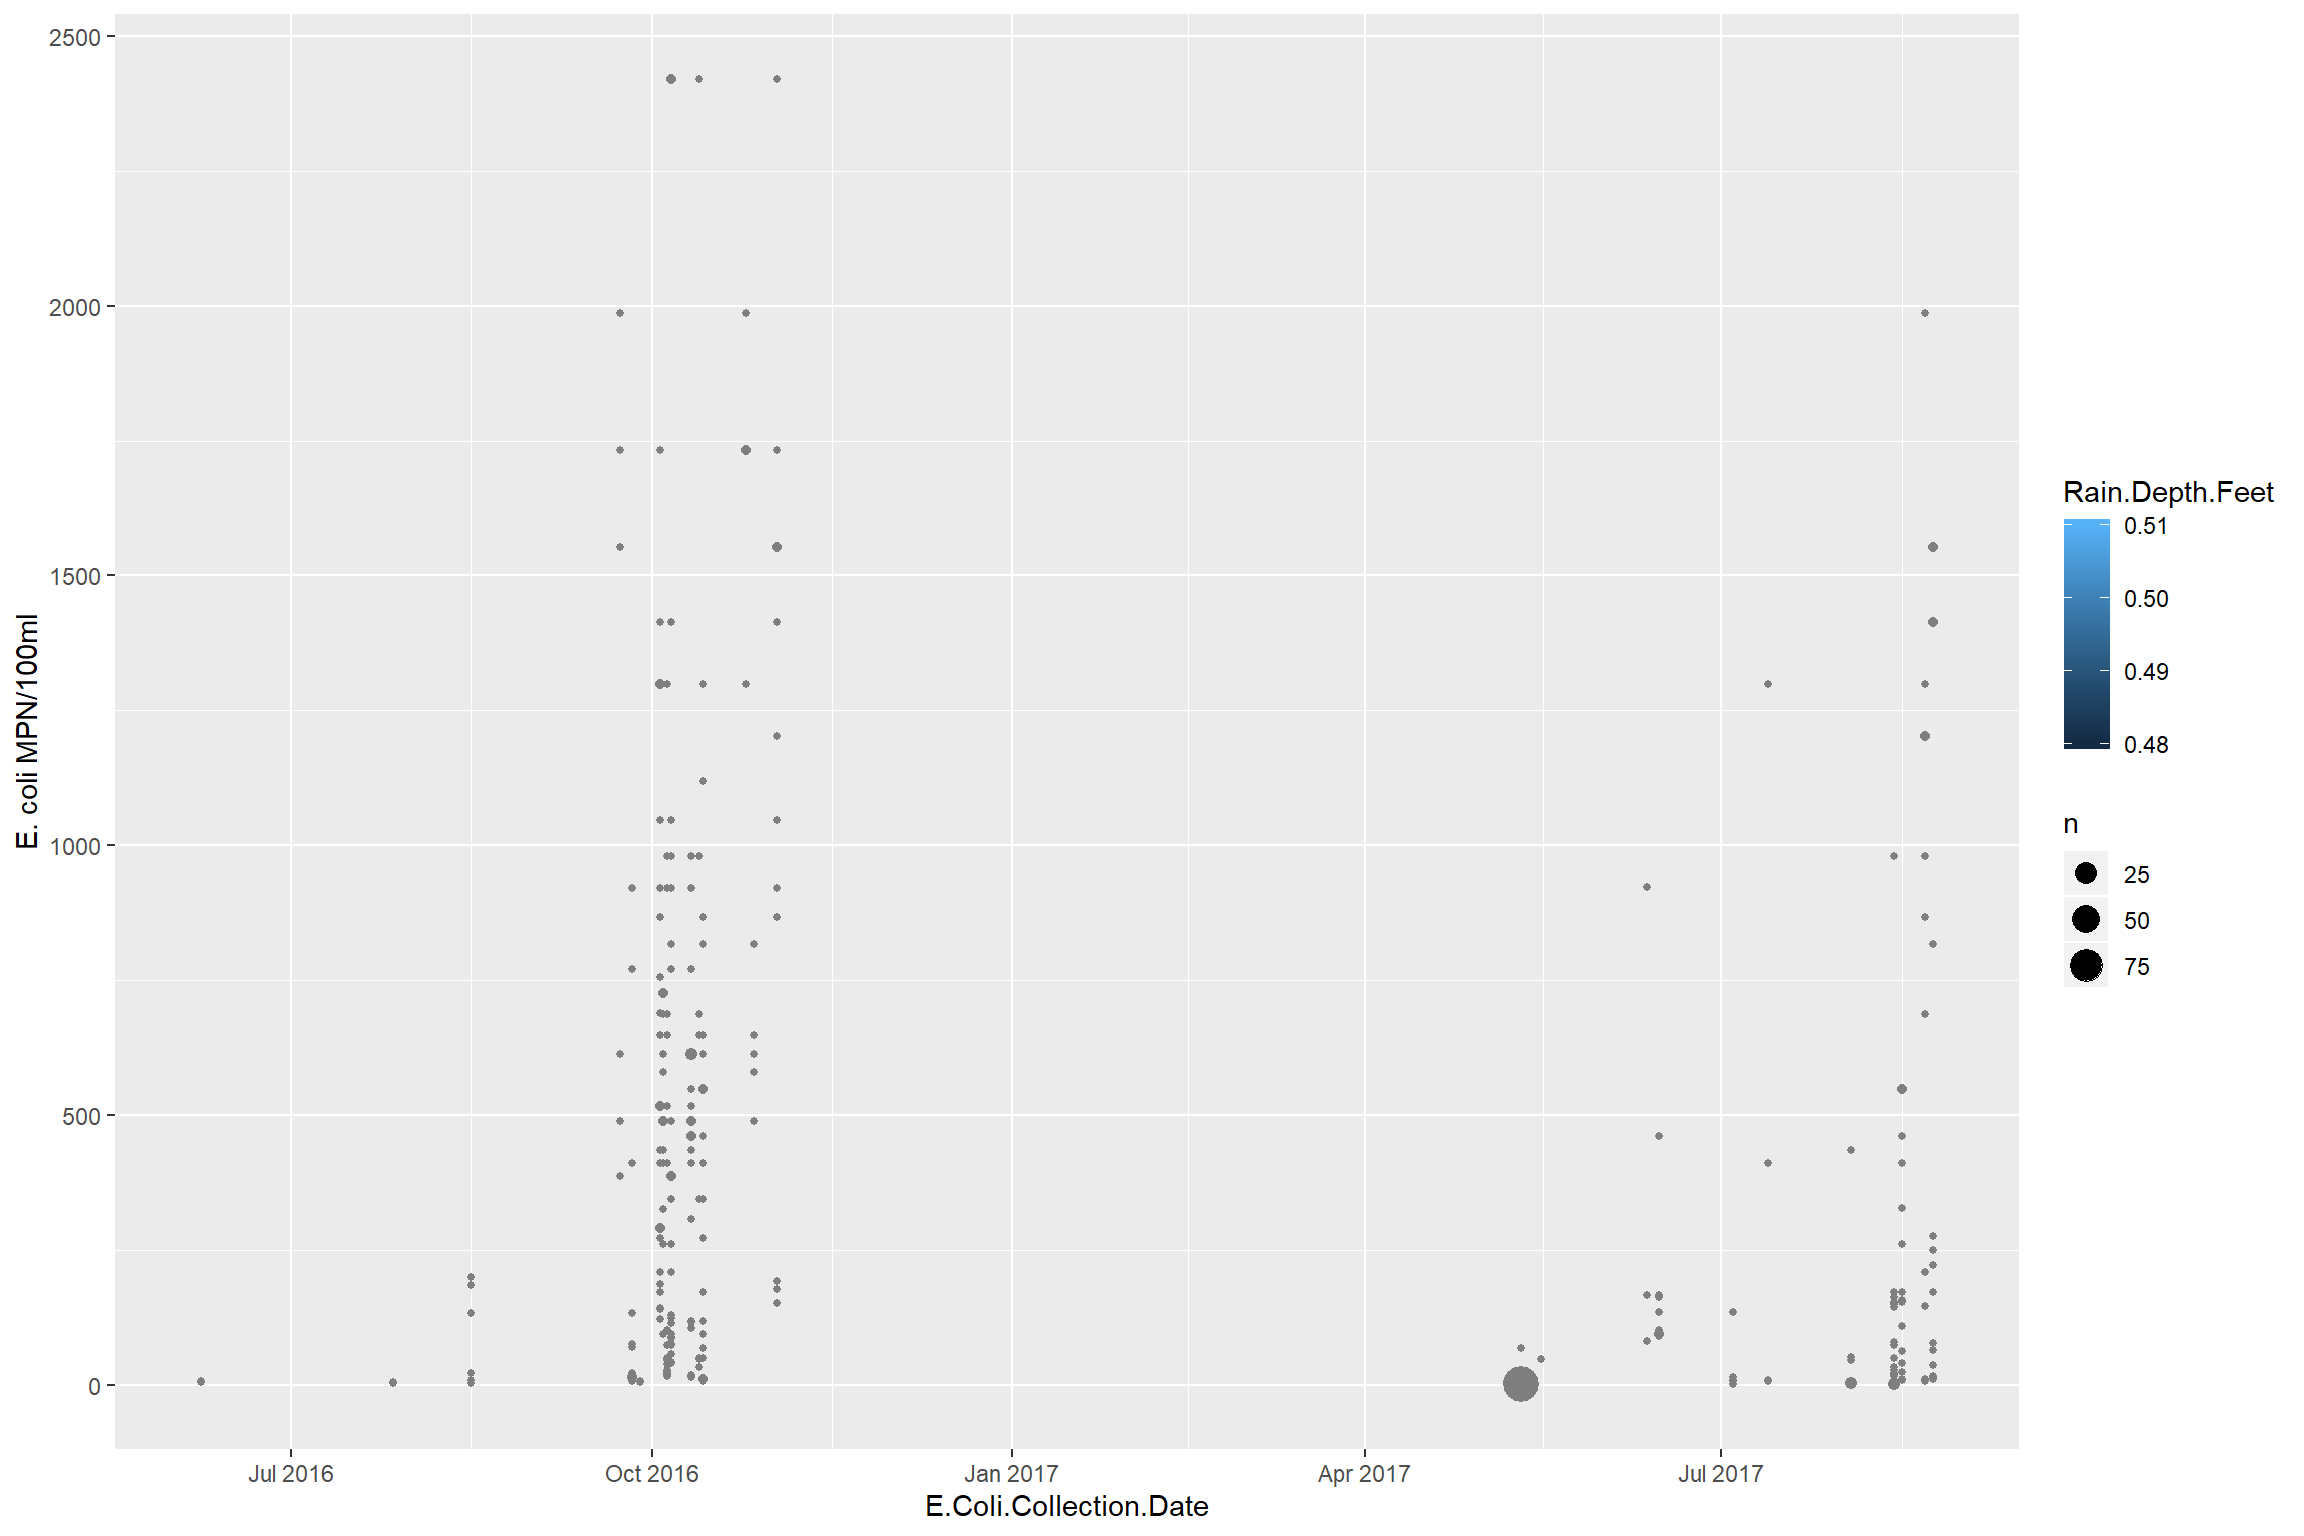
\includegraphics{Final_Project_files/figure-latex/unnamed-chunk-7-4.pdf}

\begin{Shaded}
\begin{Highlighting}[]
\KeywordTok{ggplot}\NormalTok{(df3, }\KeywordTok{aes}\NormalTok{(}\StringTok{`}\DataTypeTok{E. coli MPN/100ml}\StringTok{`}\NormalTok{)) }\OperatorTok{+}\StringTok{ }\KeywordTok{coord_cartesian}\NormalTok{(}\DataTypeTok{xlim =} \KeywordTok{c}\NormalTok{(}\DecValTok{0}\NormalTok{, }\DecValTok{4}\NormalTok{), }\DataTypeTok{ylim =} \KeywordTok{c}\NormalTok{(}\DecValTok{0}\NormalTok{, }\DecValTok{5}\NormalTok{)) }\OperatorTok{+}\StringTok{ }\KeywordTok{geom_density}\NormalTok{(}\KeywordTok{aes}\NormalTok{(}\DataTypeTok{fill=}\KeywordTok{factor}\NormalTok{(MLID)), }\DataTypeTok{alpha=}\FloatTok{0.8}\NormalTok{)}
\end{Highlighting}
\end{Shaded}

\begin{verbatim}
## Warning: Removed 5339 rows containing non-finite values (stat_density).
\end{verbatim}

\begin{verbatim}
## Warning: Groups with fewer than two data points have been dropped.

## Warning: Groups with fewer than two data points have been dropped.

## Warning: Groups with fewer than two data points have been dropped.

## Warning: Groups with fewer than two data points have been dropped.

## Warning: Groups with fewer than two data points have been dropped.

## Warning: Groups with fewer than two data points have been dropped.
\end{verbatim}

\includegraphics{Final_Project_files/figure-latex/unnamed-chunk-7-5.pdf}

\begin{Shaded}
\begin{Highlighting}[]
\KeywordTok{ggplot}\NormalTok{(df3,}\KeywordTok{aes}\NormalTok{(}\DataTypeTok{y=}\StringTok{`}\DataTypeTok{E. coli MPN/100ml}\StringTok{`}\NormalTok{, }\DataTypeTok{x=}\NormalTok{E.Coli.Collection.Date, }\DataTypeTok{color=}\NormalTok{Rain.Depth.Feet)) }\OperatorTok{+}\StringTok{ }\KeywordTok{geom_count}\NormalTok{()}
\end{Highlighting}
\end{Shaded}

\begin{verbatim}
## Warning: Removed 5339 rows containing non-finite values (stat_sum).
\end{verbatim}

\includegraphics{Final_Project_files/figure-latex/unnamed-chunk-7-6.pdf}

\begin{Shaded}
\begin{Highlighting}[]
\KeywordTok{ggplot}\NormalTok{(df3,}\KeywordTok{aes}\NormalTok{(}\DataTypeTok{y=}\StringTok{`}\DataTypeTok{E. coli MPN/100ml}\StringTok{`}\NormalTok{,}\DataTypeTok{x=}\NormalTok{Rain.Start.Date)) }\OperatorTok{+}\StringTok{ }
\StringTok{  }\KeywordTok{geom_point}\NormalTok{() }\OperatorTok{+}\StringTok{ }\KeywordTok{facet_wrap}\NormalTok{(}\OperatorTok{~}\NormalTok{MLID)}
\end{Highlighting}
\end{Shaded}

\begin{verbatim}
## Warning: Removed 5339 rows containing missing values (geom_point).
\end{verbatim}

\includegraphics{Final_Project_files/figure-latex/unnamed-chunk-7-7.pdf}

\begin{Shaded}
\begin{Highlighting}[]
\KeywordTok{ggplot}\NormalTok{(df3,}\KeywordTok{aes}\NormalTok{(}\DataTypeTok{y=}\StringTok{`}\DataTypeTok{E. coli MPN/100ml}\StringTok{`}\NormalTok{,}\DataTypeTok{x=}\NormalTok{Rain.Start.Date)) }\OperatorTok{+}\StringTok{ }
\StringTok{  }\KeywordTok{geom_line}\NormalTok{() }
\end{Highlighting}
\end{Shaded}

\begin{verbatim}
## Warning: Removed 5051 rows containing missing values (geom_path).
\end{verbatim}

\includegraphics{Final_Project_files/figure-latex/unnamed-chunk-7-8.pdf}

\begin{Shaded}
\begin{Highlighting}[]
\KeywordTok{ggplot}\NormalTok{(df3,}\KeywordTok{aes}\NormalTok{(}\DataTypeTok{y=}\NormalTok{Rain.Depth.Feet, }\DataTypeTok{x=}\NormalTok{Rain.Start.Date)) }\OperatorTok{+}\KeywordTok{geom_line}\NormalTok{()}
\end{Highlighting}
\end{Shaded}

\begin{verbatim}
## Warning: Removed 4596 rows containing missing values (geom_path).
\end{verbatim}

\includegraphics{Final_Project_files/figure-latex/unnamed-chunk-7-9.pdf}

\begin{Shaded}
\begin{Highlighting}[]
\KeywordTok{unique}\NormalTok{(df1}\OperatorTok{$}\NormalTok{Rain.Start.Date)}
\end{Highlighting}
\end{Shaded}

\begin{verbatim}
##   [1] 2017-08-24 2017-08-23 2017-08-16 2017-08-15 2017-08-03 2017-07-26
##   [7] 2017-07-19 2017-07-18 2017-07-07 2017-07-06 2017-06-29 2017-06-28
##  [13] 2017-06-26 2017-06-21 2017-06-15 2017-06-14 2017-06-12 2017-06-06
##  [19] 2017-06-05 2017-06-01 2017-05-31 2017-05-15 2017-05-08 2017-05-05
##  [25] 2017-05-03 2017-05-02 2017-05-01 2017-04-26 2017-04-25 2017-04-14
##  [31] 2017-04-10 2017-04-04 2017-03-30 2017-03-28 2017-03-17 2017-03-16
##  [37] 2017-03-14 2017-02-24 2017-02-23 2017-02-22 2017-02-06 2017-02-03
##  [43] 2017-02-02 2017-01-27 2016-12-28 2016-12-22 2016-12-20 2016-12-19
##  [49] 2016-12-15 2016-11-22 2016-11-21 2016-11-17 2016-11-16 2016-11-14
##  [55] 2016-11-09 2016-10-25 2016-10-20 2016-10-13 2016-10-12 2016-10-11
##  [61] 2016-10-05 2016-10-04 2016-09-27 2016-09-26 2016-09-21 2016-09-16
##  [67] 2016-09-14 2016-09-13 2016-09-09 2016-09-08 2016-09-07 2016-09-01
##  [73] 2016-08-29 2016-08-25 2016-08-24 2016-08-22 2016-08-16 2016-08-11
##  [79] 2016-08-10 2016-08-09 2016-08-08 2016-08-04 2016-08-03 2016-08-02
##  [85] 2016-08-01 2016-07-29 2016-07-26 2016-07-25 2016-07-20 2016-07-15
##  [91] 2016-07-12 2016-07-11 2016-07-01 2016-06-30 2016-06-28 2016-06-27
##  [97] 2016-06-24 2016-06-23 2016-06-22 2016-06-21 2016-06-14 2016-06-08
## [103] 2016-06-07 2016-05-26 2016-05-25
## 105 Levels: 2016-05-25 2016-05-26 2016-06-07 2016-06-08 ... 2017-08-24
\end{verbatim}

\begin{Shaded}
\begin{Highlighting}[]
\KeywordTok{unique}\NormalTok{(df3}\OperatorTok{$}\NormalTok{Rain.Start.Date)}
\end{Highlighting}
\end{Shaded}

\begin{verbatim}
##   [1] 2017-08-15 2017-07-06 2017-06-14 2017-04-14 2017-03-28 2016-12-19
##   [7] 2016-11-14 2016-10-04 2016-09-26 2016-08-29 2016-07-20 2016-06-21
##  [13] <NA>       2017-08-24 2017-07-07 2017-05-15 2017-01-27 2016-12-15
##  [19] 2016-11-22 2016-10-05 2016-08-08 2016-06-24 2016-05-26 2017-07-19
##  [25] 2017-06-15 2017-05-02 2017-04-04 2017-03-30 2017-02-02 2016-12-22
##  [31] 2016-11-21 2016-09-08 2016-07-26 2016-06-22 2017-07-26 2017-03-17
##  [37] 2017-02-06 2017-06-12 2017-05-01 2016-12-20 2016-06-27 2017-03-16
##  [43] 2017-02-03 2016-11-09 2016-10-13 2016-10-11 2016-09-09 2016-07-29
##  [49] 2016-06-23 2017-08-03 2017-06-28 2017-06-05 2017-06-01 2017-05-08
##  [55] 2016-10-20 2016-07-15 2017-07-18 2017-06-06 2017-05-05 2016-12-28
##  [61] 2016-11-16 2016-09-01 2016-08-01 2016-06-07 2017-08-16 2017-06-21
##  [67] 2017-05-03 2017-03-14 2016-10-12 2016-07-25 2016-11-17 2016-10-25
##  [73] 2016-09-21 2016-09-14 2016-09-13 2016-09-07 2016-08-22 2016-08-09
##  [79] 2016-07-01 2016-06-28 2017-06-26 2017-04-10 2016-08-10 2016-08-03
##  [85] 2016-05-25 2016-06-30 2016-08-11 2016-07-11 2016-06-08 2016-08-16
##  [91] 2016-07-12 2016-06-14 2017-06-29 2017-04-26 2017-02-24 2016-08-25
##  [97] 2017-02-23 2016-09-16 2016-08-02 2016-08-04 2017-08-23 2017-05-31
## [103] 2017-04-25 2017-02-22 2016-09-27 2016-08-24
## 105 Levels: 2016-05-25 2016-05-26 2016-06-07 2016-06-08 ... 2017-08-24
\end{verbatim}

\begin{Shaded}
\begin{Highlighting}[]
\NormalTok{df4 <-}\StringTok{ }\KeywordTok{filter}\NormalTok{(df3, df3}\OperatorTok{$}\NormalTok{Rain.Start.Date }\OperatorTok{==}\StringTok{ }\KeywordTok{c}\NormalTok{(}\StringTok{"2016-06-01"}\NormalTok{,}
\StringTok{"2016-06-02"}\NormalTok{,}
\StringTok{"2016-06-03"}\NormalTok{,}
\StringTok{"2016-06-04"}\NormalTok{,}
\StringTok{"2016-06-05"}\NormalTok{,}
\StringTok{"2016-06-06"}\NormalTok{,}
\StringTok{"2016-06-07"}\NormalTok{,}
\StringTok{"2016-06-08"}\NormalTok{,}
\StringTok{"2016-08-09"}\NormalTok{,}
\StringTok{"2016-08-10"}\NormalTok{,}
\StringTok{"2016-08-11"}\NormalTok{,}
\StringTok{"2016-08-12"}\NormalTok{,}
\StringTok{"2016-08-13"}\NormalTok{,}
\StringTok{"2016-08-14"}\NormalTok{,}
\StringTok{"2016-08-15"}\NormalTok{,}
\StringTok{"2016-08-16"}\NormalTok{,}
\StringTok{"2016-09-16"}\NormalTok{,}
\StringTok{"2016-09-17"}\NormalTok{,}
\StringTok{"2016-09-18"}\NormalTok{,}
\StringTok{"2016-09-19"}\NormalTok{,}
\StringTok{"2016-09-20"}\NormalTok{,}
\StringTok{"2016-09-21"}\NormalTok{,}
\StringTok{"2016-09-22"}\NormalTok{,}
\StringTok{"2016-09-23"}\NormalTok{,}
\StringTok{"2016-09-26"}\NormalTok{,}
\StringTok{"2016-09-27"}\NormalTok{,}
\StringTok{"2016-09-28"}\NormalTok{,}
\StringTok{"2016-09-29"}\NormalTok{,}
\StringTok{"2016-09-30"}\NormalTok{,}
\StringTok{"2016-10-01"}\NormalTok{, }
\StringTok{"2016-10-02"}\NormalTok{,  }
\StringTok{"2016-10-03"}\NormalTok{, }
\StringTok{"2016-10-04"}\NormalTok{, }
\StringTok{"2016-10-05"}\NormalTok{, }
\StringTok{"2016-10-06"}\NormalTok{, }
\StringTok{"2016-10-07"}\NormalTok{,}
\StringTok{"2016-10-08"}\NormalTok{,}
\StringTok{"2016-10-09"}\NormalTok{,}
\StringTok{"2016-10-10"}\NormalTok{,}
\StringTok{"2016-10-11"}\NormalTok{,}
\StringTok{"2016-10-12"}\NormalTok{,}
\StringTok{"2016-10-13"}\NormalTok{,}
\StringTok{"2016-10-14"}\NormalTok{,}
\StringTok{"2016-10-15"}\NormalTok{,}
\StringTok{"2016-10-16"}\NormalTok{,}
\StringTok{"2016-10-18"}\NormalTok{,}
\StringTok{"2016-10-19"}\NormalTok{,}
\StringTok{"2016-10-20"}\NormalTok{,}
\StringTok{"2016-10-21"}\NormalTok{,}
\StringTok{"2016-10-22"}\NormalTok{,}
\StringTok{"2016-10-23"}\NormalTok{,}
\StringTok{"2016-10-24"}\NormalTok{,}
\StringTok{"2016-10-25"}\NormalTok{,}
\StringTok{"2016-10-26"}\NormalTok{,}
\StringTok{"2016-10-27"}\NormalTok{,}
\StringTok{"2016-10-28"}\NormalTok{,}
\StringTok{"2016-10-29"}\NormalTok{,}
\StringTok{"2016-10-30"}\NormalTok{,}
\StringTok{"2016-10-31"}\NormalTok{,}
\StringTok{"2016-11-01"}\NormalTok{,}
\StringTok{"2016-11-02"}\NormalTok{,}
\StringTok{"2017-05-03"}\NormalTok{,}
\StringTok{"2017-05-04"}\NormalTok{,}
\StringTok{"2017-05-05"}\NormalTok{,}
\StringTok{"2017-05-06"}\NormalTok{, }
\StringTok{"2017-05-07"}\NormalTok{,}
\StringTok{"2017-05-08"}\NormalTok{,}
\StringTok{"2017-05-09"}\NormalTok{,}
\StringTok{"2017-05-10"}\NormalTok{,}
\StringTok{"2017-05-11"}\NormalTok{,}
\StringTok{"2017-05-12"}\NormalTok{,}
\StringTok{"2017-05-13"}\NormalTok{,}
\StringTok{"2017-05-14"}\NormalTok{,}
\StringTok{"2017-05-15"}\NormalTok{,}
\StringTok{"2017-05-16"}\NormalTok{,}
\StringTok{"2017-06-05"}\NormalTok{,}
\StringTok{"2017-06-06"}\NormalTok{,}
\StringTok{"2017-06-07"}\NormalTok{,}
\StringTok{"2017-06-08"}\NormalTok{,}
\StringTok{"2017-06-09"}\NormalTok{,}
\StringTok{"2017-06-10"}\NormalTok{,}
\StringTok{"2017-06-11"}\NormalTok{,}
\StringTok{"2017-06-12"}\NormalTok{,}
\StringTok{"2017-06-13"}\NormalTok{,}
\StringTok{"2017-06-14"}\NormalTok{,}
\StringTok{"2017-06-15"}\NormalTok{,}
\StringTok{"2017-06-27"}\NormalTok{,}
\StringTok{"2017-06-28"}\NormalTok{,}
\StringTok{"2017-06-29"}\NormalTok{,}
\StringTok{"2017-06-30"}\NormalTok{,}
\StringTok{"2017-07-01"}\NormalTok{,}
\StringTok{"2017-07-02"}\NormalTok{,}
\StringTok{"2017-07-03"}\NormalTok{,}
\StringTok{"2017-07-04"}\NormalTok{,}
\StringTok{"2017-07-06"}\NormalTok{,}
\StringTok{"2017-07-07"}\NormalTok{,}
\StringTok{"2017-07-08"}\NormalTok{,}
\StringTok{"2017-07-09"}\NormalTok{,}
\StringTok{"2017-07-10"}\NormalTok{,}
\StringTok{"2017-07-11"}\NormalTok{,}
\StringTok{"2017-07-12"}\NormalTok{,}
\StringTok{"2017-07-13"}\NormalTok{,}
\StringTok{"2017-07-05"}\NormalTok{,}
\StringTok{"2017-07-28"}\NormalTok{,}
\StringTok{"2017-07-29"}\NormalTok{,}
\StringTok{"2017-07-30"}\NormalTok{,}
\StringTok{"2017-07-31"}\NormalTok{,}
\StringTok{"2017-08-01"}\NormalTok{,}
\StringTok{"2017-08-02"}\NormalTok{,}
\StringTok{"2017-08-03"}\NormalTok{,}
\StringTok{"2017-08-07"}\NormalTok{,}
\StringTok{"2017-08-08"}\NormalTok{,}
\StringTok{"2017-08-09"}\NormalTok{,}
\StringTok{"2017-08-10"}\NormalTok{,}
\StringTok{"2017-08-11"}\NormalTok{,}
\StringTok{"2017-08-12"}\NormalTok{,}
\StringTok{"2017-08-13"}\NormalTok{,}
\StringTok{"2017-08-14"}\NormalTok{,}
\StringTok{"2017-08-15"}\NormalTok{,}
\StringTok{"2017-08-16"}\NormalTok{,}
\StringTok{"2017-08-17"}\NormalTok{,}
\StringTok{"2017-08-18"}\NormalTok{,}
\StringTok{"2017-08-19"}\NormalTok{,}
\StringTok{"2017-08-20"}\NormalTok{,}
\StringTok{"2017-08-21"}\NormalTok{,}
\StringTok{"2017-08-22"}\NormalTok{,}
\StringTok{"2017-08-23"}\NormalTok{,}
\StringTok{"2017-08-24"}\NormalTok{,}
\StringTok{"2016-07-20"}\NormalTok{,}
\StringTok{"2016-07-21"}\NormalTok{,}
\StringTok{"2016-07-22"}\NormalTok{,}
\StringTok{"2016-07-23"}\NormalTok{,}
\StringTok{"2016-07-24"}\NormalTok{,}
\StringTok{"2016-07-25"}\NormalTok{,}
\StringTok{"2016-07-26"}\NormalTok{,}
\StringTok{"2016-07-27"}\NormalTok{))}
\end{Highlighting}
\end{Shaded}

\begin{verbatim}
## Warning in `==.default`(df3$Rain.Start.Date, c("2016-06-01", "2016-06-02", :
## longer object length is not a multiple of shorter object length
\end{verbatim}

\begin{verbatim}
## Warning in is.na(e1) | is.na(e2): longer object length is not a multiple of
## shorter object length
\end{verbatim}

\begin{Shaded}
\begin{Highlighting}[]
\NormalTok{df5 <-}\StringTok{ }\KeywordTok{merge}\NormalTok{(df4,df2, }\DataTypeTok{by=}\KeywordTok{c}\NormalTok{(}\StringTok{"MLID"}\NormalTok{), }\DataTypeTok{all =} \OtherTok{TRUE}\NormalTok{)}
\end{Highlighting}
\end{Shaded}

\begin{Shaded}
\begin{Highlighting}[]
\KeywordTok{ggplot}\NormalTok{(df5,}\KeywordTok{aes}\NormalTok{(}\DataTypeTok{x=}\NormalTok{E.Coli.Collection.Date.y, }\DataTypeTok{y=}\StringTok{`}\DataTypeTok{E. coli MPN/100ml.x}\StringTok{`}\NormalTok{)) }\OperatorTok{+}
\StringTok{  }\KeywordTok{geom_line}\NormalTok{(}\KeywordTok{aes}\NormalTok{(}\DataTypeTok{col=}\NormalTok{MLID))}
\end{Highlighting}
\end{Shaded}

\begin{verbatim}
## Warning: Removed 323 rows containing missing values (geom_path).
\end{verbatim}

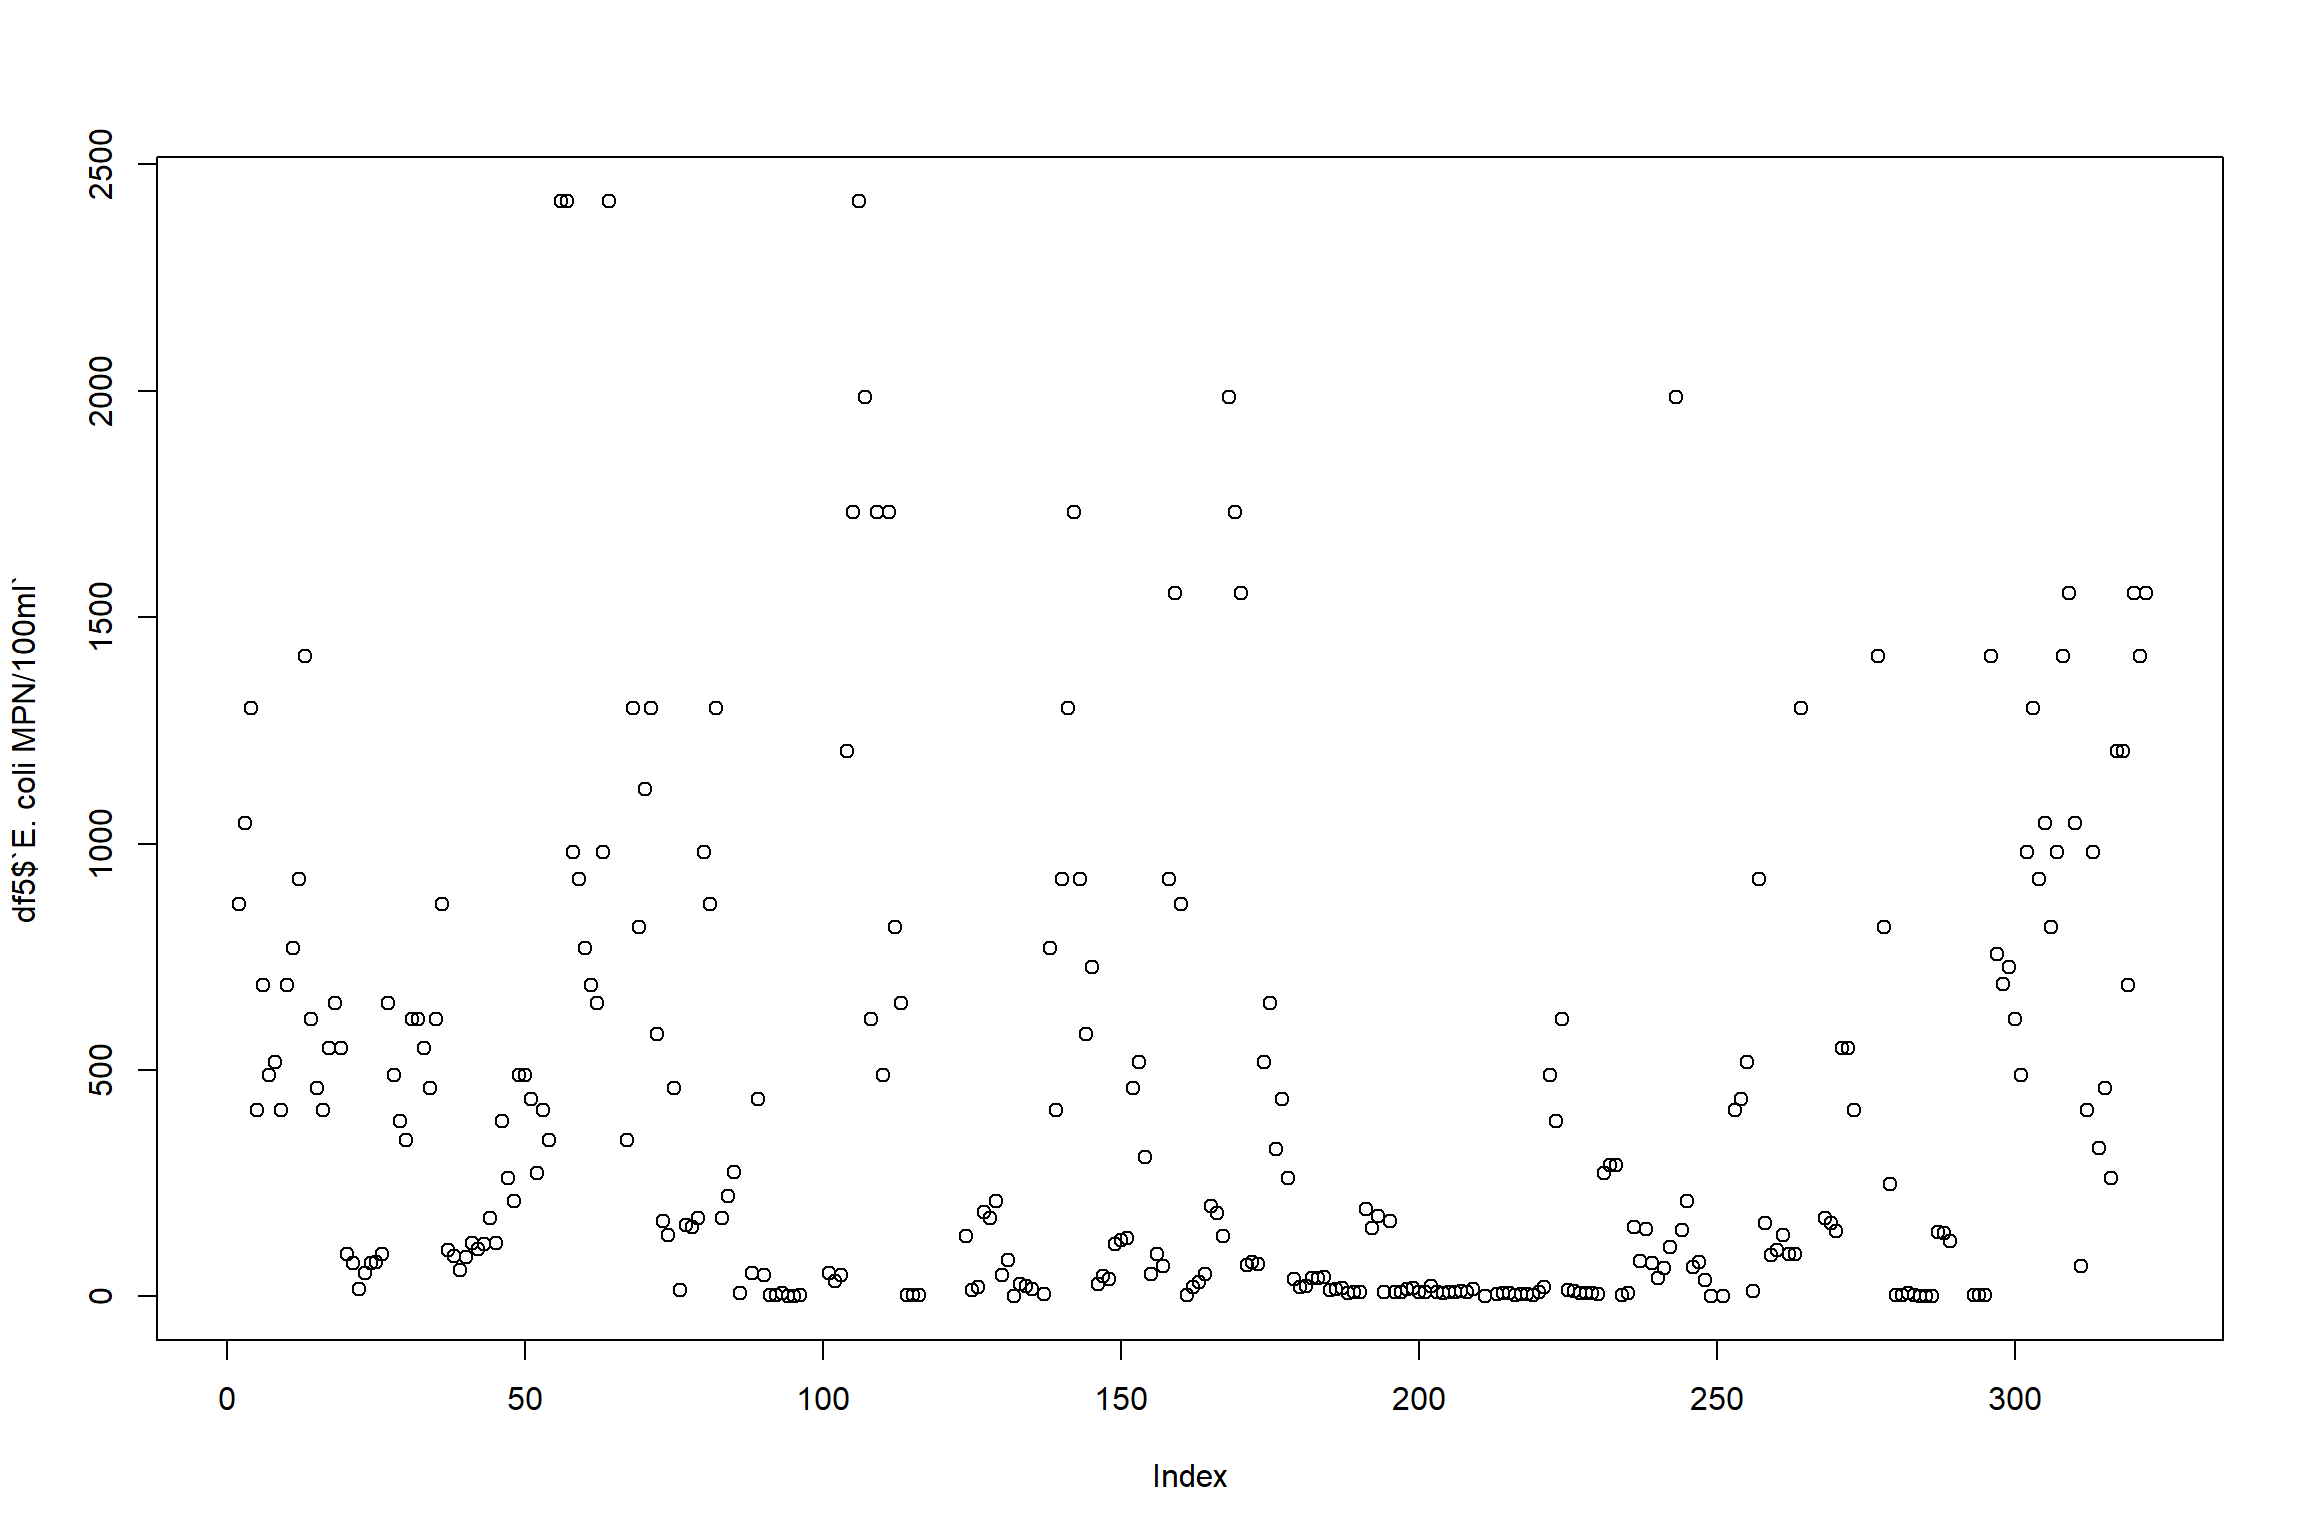
\includegraphics{Final_Project_files/figure-latex/unnamed-chunk-11-1.pdf}

\begin{Shaded}
\begin{Highlighting}[]
\KeywordTok{ggplot}\NormalTok{(df5,}\KeywordTok{aes}\NormalTok{(}\DataTypeTok{x=}\NormalTok{Rain.Start.Date, }\DataTypeTok{y=}\NormalTok{Rain.Depth.Feet)) }\OperatorTok{+}
\StringTok{  }\KeywordTok{geom_line}\NormalTok{()}
\end{Highlighting}
\end{Shaded}

\begin{verbatim}
## Warning: Removed 322 rows containing missing values (geom_path).
\end{verbatim}

\begin{verbatim}
## geom_path: Each group consists of only one observation. Do you need to adjust
## the group aesthetic?
\end{verbatim}

\includegraphics{Final_Project_files/figure-latex/unnamed-chunk-11-2.pdf}

\begin{Shaded}
\begin{Highlighting}[]
\KeywordTok{ggplot}\NormalTok{(df5,}\KeywordTok{aes}\NormalTok{(}\DataTypeTok{x=}\NormalTok{Rain.Depth.Feet, }\DataTypeTok{y=}\StringTok{`}\DataTypeTok{E. coli MPN/100ml.x}\StringTok{`}\NormalTok{)) }\OperatorTok{+}
\StringTok{  }\KeywordTok{geom_line}\NormalTok{()}
\end{Highlighting}
\end{Shaded}

\begin{verbatim}
## Warning: Removed 323 rows containing missing values (geom_path).
\end{verbatim}

\includegraphics{Final_Project_files/figure-latex/unnamed-chunk-11-3.pdf}

\begin{Shaded}
\begin{Highlighting}[]
\KeywordTok{ggplot}\NormalTok{(df3,}\KeywordTok{aes}\NormalTok{(}\DataTypeTok{x=}\NormalTok{E.Coli.Collection.Date, }\DataTypeTok{y=}\StringTok{`}\DataTypeTok{E. coli MPN/100ml}\StringTok{`}\NormalTok{)) }\OperatorTok{+}
\StringTok{  }\KeywordTok{geom_line}\NormalTok{(}\KeywordTok{aes}\NormalTok{(}\DataTypeTok{col=}\NormalTok{MLID,))}
\end{Highlighting}
\end{Shaded}

\begin{verbatim}
## Warning: Removed 5331 rows containing missing values (geom_path).
\end{verbatim}

\includegraphics{Final_Project_files/figure-latex/unnamed-chunk-11-4.pdf}

\begin{Shaded}
\begin{Highlighting}[]
\KeywordTok{ggplot}\NormalTok{(df3,}\KeywordTok{aes}\NormalTok{(}\DataTypeTok{x=}\NormalTok{Rain.Start.Date, }\DataTypeTok{y=}\NormalTok{Rain.Depth.Feet)) }\OperatorTok{+}
\StringTok{  }\KeywordTok{geom_line}\NormalTok{()}
\end{Highlighting}
\end{Shaded}

\begin{verbatim}
## Warning: Removed 4596 rows containing missing values (geom_path).
\end{verbatim}

\includegraphics{Final_Project_files/figure-latex/unnamed-chunk-11-5.pdf}

\begin{Shaded}
\begin{Highlighting}[]
\KeywordTok{ggplot}\NormalTok{(df3,}\KeywordTok{aes}\NormalTok{(}\DataTypeTok{x=}\NormalTok{Rain.Depth.Feet, }\DataTypeTok{y=}\StringTok{`}\DataTypeTok{E. coli MPN/100ml}\StringTok{`}\NormalTok{)) }\OperatorTok{+}
\StringTok{  }\KeywordTok{geom_line}\NormalTok{()}
\end{Highlighting}
\end{Shaded}

\begin{verbatim}
## Warning: Removed 5491 rows containing missing values (geom_path).
\end{verbatim}

\includegraphics{Final_Project_files/figure-latex/unnamed-chunk-11-6.pdf}

\begin{Shaded}
\begin{Highlighting}[]
\KeywordTok{ggplot}\NormalTok{(df5,}\KeywordTok{aes}\NormalTok{(}\DataTypeTok{x=}\NormalTok{LONNAD83DD.x, }\DataTypeTok{y=}\StringTok{`}\DataTypeTok{E. coli MPN/100ml.x}\StringTok{`}\NormalTok{)) }\OperatorTok{+}\KeywordTok{geom_point}\NormalTok{()}
\end{Highlighting}
\end{Shaded}

\begin{verbatim}
## Warning: Removed 323 rows containing missing values (geom_point).
\end{verbatim}

\includegraphics{Final_Project_files/figure-latex/unnamed-chunk-11-7.pdf}

\begin{Shaded}
\begin{Highlighting}[]
\KeywordTok{ggplot}\NormalTok{(df3,}\KeywordTok{aes}\NormalTok{(}\DataTypeTok{x=}\NormalTok{LONNAD83DD, }\DataTypeTok{y=}\StringTok{`}\DataTypeTok{E. coli MPN/100ml}\StringTok{`}\NormalTok{)) }\OperatorTok{+}\KeywordTok{geom_point}\NormalTok{()}
\end{Highlighting}
\end{Shaded}

\begin{verbatim}
## Warning: Removed 5339 rows containing missing values (geom_point).
\end{verbatim}

\includegraphics{Final_Project_files/figure-latex/unnamed-chunk-11-8.pdf}

\begin{Shaded}
\begin{Highlighting}[]
\KeywordTok{ggplot}\NormalTok{(df5,}\KeywordTok{aes}\NormalTok{(}\DataTypeTok{x=}\NormalTok{LATNAD83DD.x, }\DataTypeTok{y=}\StringTok{`}\DataTypeTok{E. coli MPN/100ml.x}\StringTok{`}\NormalTok{)) }\OperatorTok{+}\KeywordTok{geom_point}\NormalTok{()}
\end{Highlighting}
\end{Shaded}

\begin{verbatim}
## Warning: Removed 323 rows containing missing values (geom_point).
\end{verbatim}

\includegraphics{Final_Project_files/figure-latex/unnamed-chunk-11-9.pdf}

\begin{Shaded}
\begin{Highlighting}[]
\KeywordTok{ggplot}\NormalTok{(df3,}\KeywordTok{aes}\NormalTok{(}\DataTypeTok{x=}\NormalTok{LATNAD83DD, }\DataTypeTok{y=}\StringTok{`}\DataTypeTok{E. coli MPN/100ml}\StringTok{`}\NormalTok{)) }\OperatorTok{+}\KeywordTok{geom_point}\NormalTok{()}
\end{Highlighting}
\end{Shaded}

\begin{verbatim}
## Warning: Removed 5339 rows containing missing values (geom_point).
\end{verbatim}

\includegraphics{Final_Project_files/figure-latex/unnamed-chunk-11-10.pdf}

\end{document}
